
\begin{figure}[t!]
    \centering
    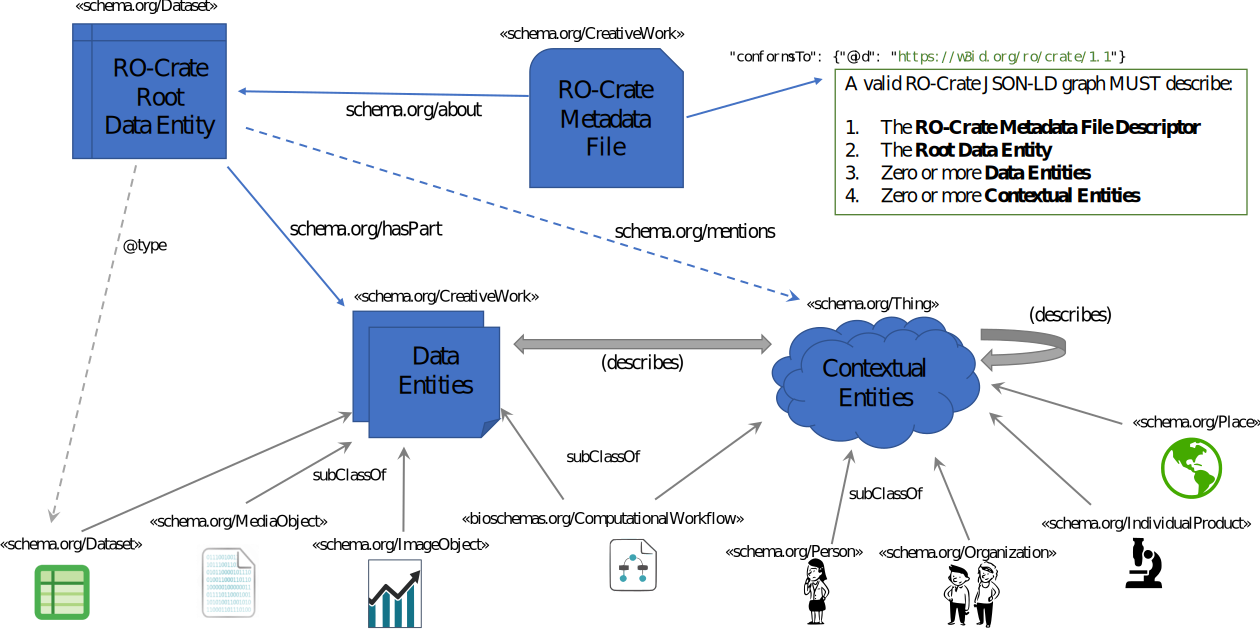
\includegraphics[width=0.9\textwidth]{content/images/ro-crate-uml.pdf}
    \caption{\textbf{Simplified UML class diagram of RO-Crate.} The \emph{RO-Crate Metadata File} conforms to a version of the specification; and contains a JSON-LD graph that describes the entities that make up the RO-Crate. The \emph{RO-Crate Root Data Entity} represent the Research Object as a dataset. The RO-Crate aggregates \emph{data entities} (\texttt{hasPart}) which are further described using \emph{contextual entities} (which may include aggregated and non-aggregated data entities). Multiple types and relations from Schema.org allow annotations to be more specific, including figures, nested datasets, computational workflows, people, organisations, instruments and places. Contextual entities not otherwise cross-referenced from other entities' properties (\emph{describes}) can be grouped under the root entity (\texttt{mentions}).}
    \label{fig:uml}
\end{figure}
